\documentclass[aspectratio=169]{beamer}
\usetheme{Madrid}
\usecolortheme{default}

% Packages
\usepackage{graphicx}
\usepackage{listings}
\usepackage{xcolor}
\usepackage{tikz}
\usetikzlibrary{positioning,arrows.meta,shapes.geometric}
\usepackage{hyperref}

% Colors
\definecolor{codegreen}{rgb}{0,0.6,0}
\definecolor{codegray}{rgb}{0.5,0.5,0.5}
\definecolor{codepurple}{rgb}{0.58,0,0.82}
\definecolor{backcolour}{rgb}{0.95,0.95,0.92}

% Code listing style
\lstdefinestyle{mystyle}{
    backgroundcolor=\color{backcolour},   
    commentstyle=\color{codegreen},
    keywordstyle=\color{magenta},
    numberstyle=\tiny\color{codegray},
    stringstyle=\color{codepurple},
    basicstyle=\ttfamily\footnotesize,
    breakatwhitespace=false,         
    breaklines=true,                 
    captionpos=b,                    
    keepspaces=true,                 
    numbers=left,                    
    numbersep=5pt,                  
    showspaces=false,                
    showstringspaces=false,
    showtabs=false,                  
    tabsize=2
}
\lstset{style=mystyle}

% Title page information
\title{5G Network Simulation with Secure Syslog Integration}
\subtitle{Midterm Presentation}
\author{Rishabh Kumar (cs25resch04002)}
\institute{WNS}
\date{November 2025}

\begin{document}

% Title slide
\begin{frame}
\titlepage
\end{frame}

% Table of contents
\begin{frame}{Outline}
\tableofcontents
\end{frame}

% Section 1: Introduction
\section{Introduction}

\begin{frame}{Project Overview}
\begin{itemize}
    \item \textbf{Goal:} Implement a comprehensive 5G network simulation with secure logging infrastructure
    \item \textbf{Key Components:}
    \begin{itemize}
        \item 5G Standalone (SA) network using OpenAirInterface
        \item UE Location Service for tracking devices
        \item Secure syslog integration with TLS encryption
    \end{itemize}
    \item \textbf{Use Cases:}
    \begin{itemize}
        \item Network monitoring and analysis
        \item Security audit and compliance
        \item Real-time location tracking
    \end{itemize}
\end{itemize}
\end{frame}

\begin{frame}{Motivation}
\begin{columns}
\column{0.5\textwidth}
\textbf{Challenges in 5G Networks:}
\begin{itemize}
    \item Complex architecture
    \item Security concerns
    \item Log management at scale
    \item Real-time monitoring needs
\end{itemize}

\column{0.5\textwidth}
\textbf{Our Solution:}
\begin{itemize}
    \item Simulated 5G environment
    \item Centralized secure logging
    \item Location tracking service
    \item Automated analysis tools
\end{itemize}
\end{columns}
\end{frame}

% Section 2: 5G Network Simulation
\section{5G Network Simulation}

\begin{frame}{5G Architecture}
\begin{center}
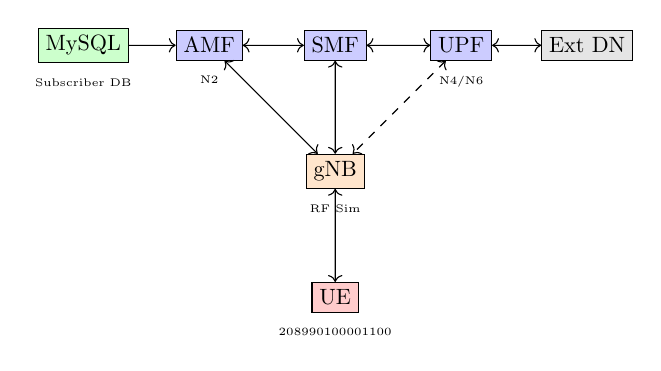
\begin{tikzpicture}[scale=0.8, every node/.style={scale=0.8}]
    % Core Network
    \node[draw, rectangle, fill=blue!20] (amf) at (0,2) {AMF};
    \node[draw, rectangle, fill=blue!20] (smf) at (2,2) {SMF};
    \node[draw, rectangle, fill=blue!20] (upf) at (4,2) {UPF};
    \node[draw, rectangle, fill=green!20] (mysql) at (-2,2) {MySQL};
    
    % RAN
    \node[draw, rectangle, fill=orange!20] (gnb) at (2,0) {gNB};
    
    % UE
    \node[draw, rectangle, fill=red!20] (ue) at (2,-2) {UE};
    
    % External
    \node[draw, rectangle, fill=gray!20] (dn) at (6,2) {Ext DN};
    
    % Connections
    \draw[->] (mysql) -- (amf);
    \draw[<->] (amf) -- (smf);
    \draw[<->] (smf) -- (upf);
    \draw[<->] (upf) -- (dn);
    \draw[<->] (amf) -- (gnb);
    \draw[<->] (smf) -- (gnb);
    \draw[<->] (gnb) -- (ue);
    \draw[<->, dashed] (upf) -- (gnb);
    
    % Labels
    \node[below=0.1cm of mysql] {\tiny Subscriber DB};
    \node[below=0.1cm of amf] {\tiny N2};
    \node[below=0.1cm of upf] {\tiny N4/N6};
    \node[below=0.1cm of gnb] {\tiny RF Sim};
    \node[below=0.1cm of ue] {\tiny 208990100001100};
\end{tikzpicture}
\end{center}
\end{frame}

\begin{frame}{Network Configuration}
\begin{columns}
\column{0.5\textwidth}
\textbf{Control Plane (Public Net)}
\begin{itemize}
    \item Subnet: 192.168.71.128/26
    \item MySQL: .131
    \item AMF: .132
    \item SMF: .133
    \item UPF: .134
    \item gNB: .140
    \item UE: .150
\end{itemize}

\column{0.5\textwidth}
\textbf{User Plane (Traffic Net)}
\begin{itemize}
    \item Subnet: 192.168.72.128/26
    \item UPF: .134
    \item External DN: .135
    \item Protocols: GTP-U
\end{itemize}
\end{columns}
\vspace{0.5cm}
\textbf{Technologies:} Docker, OpenAirInterface v2.1.10, RF Simulator
\end{frame}

\begin{frame}[fragile]{Deployment Process}
\begin{lstlisting}[language=bash, caption=Network Setup Commands]
# Create Docker networks
docker network create --subnet=192.168.71.128/26 \
  rfsim5g-oai-public-net
docker network create --subnet=192.168.72.128/26 \
  rfsim5g-oai-traffic-net

# Deploy 5G Core
docker-compose up -d mysql oai-amf oai-smf \
  oai-upf oai-ext-dn

# Deploy RAN
docker-compose up -d oai-gnb

# Deploy UE
docker-compose up -d oai-nr-ue
\end{lstlisting}
\end{frame}

\begin{frame}{Verification Results}
\begin{block}{gNB Connection Status}
\texttt{Status: Connected | Global Id: 0x0E00 | gNB Name: gnb-rfsim}
\end{block}

\begin{block}{UE Registration}
\texttt{5GMM-REGISTERED | IMSI: 208990100001100 | Cell: 0000e014e}
\end{block}

\begin{block}{Connectivity Test}
\texttt{5 packets transmitted, 5 received, 0\% packet loss}
\end{block}

\begin{alertblock}{Achievement}
$\checkmark$ Full 5G SA network operational with end-to-end connectivity
\end{alertblock}
\end{frame}

% Section 3: UE Location Service
\section{UE Location Service}

\begin{frame}{Location Service Architecture}
\begin{center}
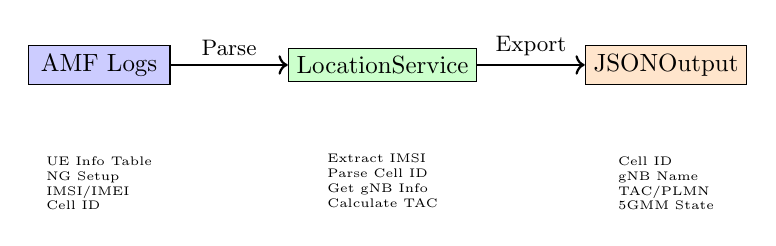
\begin{tikzpicture}[scale=0.9, every node/.style={scale=0.9}]
    % Components
    \node[draw, rectangle, fill=blue!20, minimum width=2cm] (amf) at (0,2) {AMF Logs};
    \node[draw, rectangle, fill=green!20, minimum width=2cm] (service) at (4,2) {Location\\Service};
    \node[draw, rectangle, fill=orange!20, minimum width=2cm] (output) at (8,2) {JSON\\Output};
    
    % Data flow
    \draw[->, thick] (amf) -- node[above] {\small Parse} (service);
    \draw[->, thick] (service) -- node[above] {\small Export} (output);
    
    % Details
    \node[below=0.8cm of amf, align=left, font=\tiny] {
        UE Info Table\\
        NG Setup\\
        IMSI/IMEI\\
        Cell ID
    };
    
    \node[below=0.8cm of service, align=left, font=\tiny] {
        Extract IMSI\\
        Parse Cell ID\\
        Get gNB Info\\
        Calculate TAC
    };
    
    \node[below=0.8cm of output, align=left, font=\tiny] {
        Cell ID\\
        gNB Name\\
        TAC/PLMN\\
        5GMM State
    };
\end{tikzpicture}
\end{center}
\end{frame}

\begin{frame}[fragile]{Location Service Implementation}
\begin{lstlisting}[language=Python, caption=Key Functions]
class UELocationService:
    def get_amf_logs(self):
        """Fetch AMF container logs"""
        cmd = ["docker", "logs", "rfsim5g-oai-amf"]
        result = subprocess.run(cmd, capture_output=True)
        return result.stdout.decode('utf-8')
    
    def get_ue_location_by_imsi(self, imsi):
        """Extract UE location from AMF logs"""
        logs = self.get_amf_logs()
        # Parse UE info table
        ue_info = self.parse_ue_info_table(logs, imsi)
        # Parse gNB information
        gnb_info = self.parse_ng_setup_request(logs)
        return {
            'ue_identity': ue_info,
            'network_location': {...},
            'gnb_info': gnb_info
        }
\end{lstlisting}
\end{frame}

\begin{frame}{Location Data Extracted}
\begin{columns}
\column{0.5\textwidth}
\textbf{UE Identity:}
\begin{itemize}
    \item IMSI: 208990100001100
    \item GUTI
    \item RAN UE NGAP ID
    \item AMF UE NGAP ID
\end{itemize}

\textbf{Network Location:}
\begin{itemize}
    \item Cell ID: 0000e014e
    \item TAC: 00 00 01
    \item PLMN: MCC=208, MNC=99
\end{itemize}

\column{0.5\textwidth}
\textbf{gNB Information:}
\begin{itemize}
    \item gNB ID: 0x0E00
    \item gNB Name: gnb-rfsim
    \item Status: Connected
\end{itemize}

\textbf{Registration State:}
\begin{itemize}
    \item 5GMM State: REGISTERED
    \item UE IP: 12.1.1.2
\end{itemize}
\end{columns}

\vspace{0.5cm}
\textbf{Note:} All data extracted from real AMF logs, no mock data used
\end{frame}

\begin{frame}[fragile]{Usage Examples}
\begin{lstlisting}[language=bash, caption=Location Service Commands]
# Get location by IMSI
python3 ue_location_service.py --imsi 208990100001100

# Get location by IMEI
python3 ue_location_service.py --imei 862104052096703

# Get all UE locations
python3 ue_location_service.py --all

# Export to JSON
python3 ue_location_service.py --imsi 208990100001100 \
  --export ue_location.json
\end{lstlisting}
\end{frame}

% Section 4: Secure Syslog Integration
\section{Secure Syslog Integration}

\begin{frame}{Secure Syslog Architecture}
\begin{center}
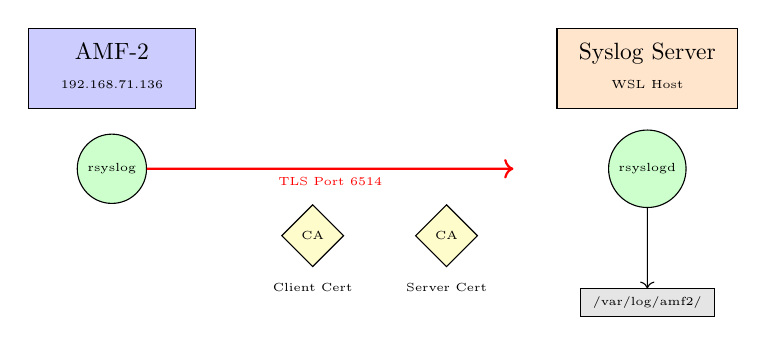
\begin{tikzpicture}[scale=0.85, every node/.style={scale=0.85}]
    % AMF-2
    \node[draw, rectangle, fill=blue!20, minimum width=2.5cm, minimum height=1.2cm] (amf2) at (0,0) {
        \begin{tabular}{c}
        AMF-2\\
        \tiny 192.168.71.136
        \end{tabular}
    };
    
    % Rsyslog in AMF-2
    \node[draw, circle, fill=green!20, minimum size=0.8cm] (rsyslog1) at (0,-1.5) {\tiny rsyslog};
    
    % TLS Tunnel
    \draw[->, thick, red] (rsyslog1) -- node[below, sloped] {\tiny TLS Port 6514} (6,-1.5);
    
    % Syslog Server
    \node[draw, rectangle, fill=orange!20, minimum width=2.5cm, minimum height=1.2cm] (server) at (8,0) {
        \begin{tabular}{c}
        Syslog Server\\
        \tiny WSL Host
        \end{tabular}
    };
    
    % Rsyslog Server
    \node[draw, circle, fill=green!20, minimum size=0.8cm] (rsyslog2) at (8,-1.5) {\tiny rsyslogd};
    
    % Certificate indicators
    \node[draw, diamond, fill=yellow!20, minimum size=0.5cm] (cert1) at (3,-2.5) {\tiny CA};
    \node[below=0.1cm of cert1, font=\tiny] {Client Cert};
    
    \node[draw, diamond, fill=yellow!20, minimum size=0.5cm] (cert2) at (5,-2.5) {\tiny CA};
    \node[below=0.1cm of cert2, font=\tiny] {Server Cert};
    
    % Log file
    \node[draw, rectangle, fill=gray!20, minimum width=2cm] (logfile) at (8,-3.5) {\tiny /var/log/amf2/};
    \draw[->] (rsyslog2) -- (logfile);
\end{tikzpicture}
\end{center}
\end{frame}

\begin{frame}{Security Implementation}
\begin{block}{TLS Certificate Chain}
\begin{itemize}
    \item \textbf{CA Certificate:} Self-signed root CA (CN=Syslog CA)
    \item \textbf{Server Certificate:} CN=syslog-server
    \item \textbf{Client Certificate:} CN=amf-2
    \item \textbf{Key Size:} RSA 4096-bit
    \item \textbf{Validity:} 365 days
\end{itemize}
\end{block}

\begin{block}{Authentication}
\begin{itemize}
    \item x509/name authentication mode
    \item Mutual TLS verification
    \item Certificate CN validation
    \item Only authorized clients (CN=amf-2) permitted
\end{itemize}
\end{block}
\end{frame}

\begin{frame}[fragile]{Rsyslog Configuration}
\begin{lstlisting}[caption=Syslog Server Config (/etc/rsyslog.d/99-amf-secure.conf)]
# Load TLS module
module(load="imtcp"
       StreamDriver.Name="gtls"
       StreamDriver.Mode="1"
       StreamDriver.Authmode="x509/name")

# Global TLS settings
global(
    DefaultNetstreamDriver="gtls"
    DefaultNetstreamDriverCAFile="/path/to/ca-cert.pem"
    DefaultNetstreamDriverCertFile="/path/to/server-cert.pem"
    DefaultNetstreamDriverKeyFile="/path/to/server-key.pem"
)

# Accept connections on port 6514
input(type="imtcp" port="6514" ruleset="amf2"
      StreamDriver.Name="gtls"
      PermittedPeer=["amf-2"])
\end{lstlisting}
\end{frame}

\begin{frame}{AMF-2 Deployment}
\begin{columns}
\column{0.5\textwidth}
\textbf{Container Configuration:}
\begin{itemize}
    \item Image: oai-amf:v2.1.10
    \item IP: 192.168.71.136
    \item AMF Set ID: 002
    \item N2 Port: 38413
\end{itemize}

\textbf{Certificates Mounted:}
\begin{itemize}
    \item CA certificate
    \item Client certificate
    \item Client private key
\end{itemize}

\column{0.5\textwidth}
\textbf{Log Forwarding:}
\begin{itemize}
    \item Target: WSL host
    \item Port: 6514
    \item Protocol: TCP over TLS
    \item Format: RFC 5424
\end{itemize}

\textbf{Custom Entrypoint:}
\begin{itemize}
    \item Install rsyslog
    \item Configure TLS
    \item Start rsyslogd
    \item Launch AMF
\end{itemize}
\end{columns}
\end{frame}

\begin{frame}{Verification Results}
\begin{block}{Syslog Server Status}
\texttt{rsyslogd listening on 0.0.0.0:6514 (TLS enabled)}
\end{block}

\begin{block}{AMF-2 Connection}
\texttt{TLS handshake successful | Peer verified: CN=amf-2}
\end{block}

\begin{block}{Log Reception}
\texttt{/var/log/amf2/amf2-2025-11-10.log created}\\
\texttt{566 bytes received from 192.168.71.136}
\end{block}

\begin{alertblock}{Achievement}
$\checkmark$ Secure syslog operational with TLS encryption and authentication
\end{alertblock}
\end{frame}

% Section 5: Results & Analysis
\section{Results \& Analysis}

\begin{frame}{Implementation Summary}
\begin{table}
\centering
\begin{tabular}{|l|c|}
\hline
\textbf{Component} & \textbf{Status} \\
\hline
5G Core (MySQL, AMF, SMF, UPF) & $\checkmark$ Running \\
gNB (RF Simulator) & $\checkmark$ Connected \\
UE (RF Simulator) & $\checkmark$ Registered \\
End-to-End Connectivity & $\checkmark$ Verified \\
UE Location Service & $\checkmark$ Operational \\
Secure Syslog Server & $\checkmark$ Running \\
AMF-2 with Syslog & $\checkmark$ Forwarding \\
TLS Authentication & $\checkmark$ Verified \\
\hline
\end{tabular}
\caption{System Component Status}
\end{table}
\end{frame}

\begin{frame}{Key Achievements}
\begin{enumerate}
    \item \textbf{5G Network Simulation}
    \begin{itemize}
        \item Deployed complete 5G SA network using OpenAirInterface
        \item Successfully registered UE with 0\% packet loss
        \item Verified all protocols (NGAP, PFCP, GTP-U, SCTP)
    \end{itemize}
    
    \item \textbf{UE Location Service}
    \begin{itemize}
        \item Built Python service to extract location from AMF logs
        \item Support for IMSI/IMEI-based queries
        \item JSON export functionality
        \item Real data only, no mock coordinates
    \end{itemize}
    
    \item \textbf{Secure Syslog Integration}
    \begin{itemize}
        \item Deployed AMF-2 with TLS-encrypted log forwarding
        \item Implemented x509 certificate authentication
        \item Verified secure log transmission and storage
    \end{itemize}
\end{enumerate}
\end{frame}

\begin{frame}{Technical Challenges \& Solutions}
\begin{columns}
\column{0.5\textwidth}
\textbf{Challenges:}
\begin{enumerate}
    \item Docker compose compatibility
    \item IMEI extraction from logs
    \item TLS certificate validation
    \item Container networking
\end{enumerate}

\column{0.5\textwidth}
\textbf{Solutions:}
\begin{enumerate}
    \item Modified YAML config
    \item Regex pattern matching
    \item Proper CN configuration
    \item External network setup
\end{enumerate}
\end{columns}

\vspace{0.5cm}
\begin{alertblock}{Lesson Learned}
Thorough log analysis and proper certificate management are crucial for secure 5G deployments
\end{alertblock}
\end{frame}

% Section 6: Conclusion
\section{Conclusion \& Future Work}

\begin{frame}{Project Deliverables}
\begin{itemize}
    \item $\checkmark$ \textbf{Working 5G network} with OAI (7 containers)
    \item $\checkmark$ \textbf{UE Location Service} (Python script with full documentation)
    \item $\checkmark$ \textbf{Secure Syslog Server} with TLS encryption
    \item $\checkmark$ \textbf{AMF-2 Deployment} with log forwarding
    \item $\checkmark$ \textbf{Documentation:} README, setup guides, API docs
    \item $\checkmark$ \textbf{Git Repository:} 4 commits with version control
\end{itemize}

\vspace{0.5cm}
\textbf{Repository:} github.com/username/WNS (to be pushed)\\
\textbf{Lines of Code:} 1500+ (Python, YAML, Shell, Config)
\end{frame}

\begin{frame}{Future Enhancements}
\begin{enumerate}
    \item \textbf{Advanced Monitoring}
    \begin{itemize}
        \item Real-time dashboard (Grafana/Kibana)
        \item ML-based anomaly detection
        \item Automated alerting system
    \end{itemize}
    
    \item \textbf{Scalability}
    \begin{itemize}
        \item Multi-UE scenarios (10+ devices)
        \item Load balancing across AMFs
        \item Kubernetes deployment
    \end{itemize}
    
    \item \textbf{Security}
    \begin{itemize}
        \item SIEM integration
        \item Threat detection rules
        \item Compliance reporting
    \end{itemize}
    
    \item \textbf{Geographic Features}
    \begin{itemize}
        \item Cell database integration
        \item Real GPS coordinates
        \item Location visualization
    \end{itemize}
\end{enumerate}
\end{frame}

\begin{frame}{References}
\begin{thebibliography}{99}
\bibitem{3gpp}
3GPP TS 23.501: System Architecture for the 5G System

\bibitem{oai}
OpenAirInterface Software Alliance
\url{https://openairinterface.org/}

\bibitem{rfc5424}
RFC 5424: The Syslog Protocol

\bibitem{rfc5425}
RFC 5425: Transport Layer Security (TLS) Transport Mapping for Syslog

\bibitem{docker}
Docker Documentation
\url{https://docs.docker.com/}
\end{thebibliography}
\end{frame}

\begin{frame}[plain]
\centering
\vspace{2cm}
\Huge Thank You!

\vspace{1cm}
\Large
\textbf{Questions?}

\vspace{1.5cm}
\normalsize
Rishabh Kumar (cs25resch04002)\\
kumarrishabh73@gmail.com
\end{frame}

\end{document}
